\documentclass[../thesis.tex]{subfiles}
\begin{document}
\chapter{Technologies and Toolset}

\section{Server Technologies}
\subsection{Node}
The official website (http://www.nodejs.org) defines Node as "a platform built on Chrome's JavaScript runtime for easily building fast, scalable network applications. Node.js uses an event-driven, non-blocking I/O model that makes it lightweight and efficient, perfect for data-intensive real-time applications that run across distributed devices [1]."
\paragraph{}
Regardless, JavaScript is the world's most famous programming languages. If you have done any programming for the web, it's unavoidable. JavaScript, in view of the sheer reach of the web, has satisfied the "compose once, run anywhere" dream that Java had back in the 1990s.  
Around the season of the Ajax insurgency in 2005, JavaScript went from being a "toy" language to something individuals wrote genuine and noteworthy projects with. A portion of the eminent firsts were Google Maps and Gmail, yet today there are a large group of web applications from Twitter to Facebook to GitHub.
\paragraph{}

JavaScript has for some time been the true standard for frontend side web development. While about all frontend code is composed in JavaScript, server-side development is a variety of choices between PHP, Java, and various different technologies. Life as a web engineer would be substantially more straightforward if a single language was utilized all around. Since JavaScript overwhelms in the browser, it bodes well to utilize it on the server too. 
\paragraph{}

The idea of server-side JavaScript is not a new one. Netscape initially introduced JavaScript into the server world in 1994. Since that time, a lot of projects have endeavoured, and failed, to advance JavaScript as a server-side language. Execution, or scarcity thereof, restricted JavaScript from picking up a genuine a dependable balance in the server space. 
\paragraph{}

Throughout the years, JavaScript has seen gigantic upgrades in performance. Because of its pertinence in the program, enormous players like Google have contributed a considerable measure of time and cash to make JavaScript as fast as possible. In 2009, Ryan Dahl of Joyent, put the large part of that recently discovered execution to great use on the server when he made the Node.js structure. Dahl assembled Node.js over Google's V8 JavaScript engine. V8 is a similar engine that has given Google Chrome its astounding JavaScript performance, and helped it turn into the most well-known browser on the planet.
\newpage
\subsection*{Technical Details}
\begin{itemize}
    \item \textbf{Threading}
    \paragraph{}
    Node.js works in a single threaded environment, utilizing non-blocking I/O calls, enabling it to support a huge number of simultaneous connections without incurring the cost of thread context switching [17]. The idea of sharing a single thread among every one of the requests that utilization the observer design is for building exceptionally concurrent applications, where any function performing I/O must utilize a callback. With a specific end goal to accommodate the single-threaded event loop, Node.js uses the libuv library that, utilizes a fixed-sized thread pool that is in charge of a portion of the non-blocking async I/O operations [18].
    \paragraph{}
    A drawback of this single-threaded approach is that Node.js does not permit vertical scaling by increasing the amount of CPU cores of the machine it's running on while not using a further module, like cluster, StrongLoop process Manager, or pm2. However, developers can increase the default range of threads within the libuv thread pool; these threads are probably to be distributed across multiple cores by the server software system [19].
    \paragraph{}
    Execution of concurrent tasks in Node.js is handled by a thread pool. the main thread decision functions post tasks to the shared task queue that threads within the thread pool pull and execute. Inherently non-blocking system functions like networking interprets to kernel-side non-blocking sockets, whereas inherently blocking system functions like file I/O run in an exceedingly block method on its own thread When a thread in the thread pool completes a task, it informs the main thread of this, which wakes up and execute the callback. As callbacks are handled synchronously on the main thread, long lasting computations and other CPU-bound tasks will freeze the whole event-loop till completion.
    \paragraph{}
    \item \textbf{V8 Engine}
    \paragraph{}
    V8 is the JavaScript execution engine built for Google Chrome and open-sourced by Google in 2008. Written in C++, V8 compiles JavaScript source code to native machine code instead of interpreting it in real time [18].
    \paragraph{}
    Node.js makes use of libuv to handle asynchronous events. Libuv is an abstraction layer file system and network functionality on each Windows and POSIX-based systems like UNIX operating system, macOS, OSS on NonStop, and Unix.
    \paragraph{}
    The core functionality of Node.js resides in a JavaScript library. The Node.js bindings, written in C++, connect these technologies to each other and to the operating system.
    \paragraph{}
    \item \textbf{Package Management}
    \paragraph{}
    npm is an in-built package manager for the Node.js servers. It is utilized to install Node.js programs from the npm registry, sorting out the installation and administration of third-party Node.js programs. npm isn't to be mistaken for the CommonJS ‘require()’ statement. It is not utilized to load code; rather, it is utilized to install code and manage dependencies from the command line. The bundles found in the npm registry can extend from basic helper libraries, for example, Lodash to task runners suck as Gulp.
    \paragraph{}
    \item \textbf{Unified API}
    \paragraph{}
    Node.js may be combined with a browser, a database supporting JSON information (such as Postgres, MongoDB, or CouchDB) and JSON for a unified JavaScript development stack. With the difference of what were basically server-side development patterns like MVC, MVP, MVVM, etc., Node.js permits the reuse of the same model and service interface between client-side and server-side.
    \paragraph{}
    \item \textbf{Event Loop}
    \paragraph{}
    Node.js registers itself with the software system so as to be notified once a connection is created, and also the OS can issue a callback. inside the Node.js runtime, every connection could be a small heap allocation. historically, comparatively heavyweight OS processes or threads handled every connection. Node.js uses an event loop for scalability, rather than processes or threads [74]. In distinction to different event-driven servers, Node.js's event loop doesn't need to be known as explicitly. Instead callbacks are outlined, and also the server mechanically enters the event loop at the end of the callback definition. Node.js exits the event loop once there are not any any callbacks to be performed.
    \paragraph{}
    \item \textbf{Non-blocking}
    \paragraph{}
    The question of whether an operation is blocking or non-blocking refers to the fact that it must finish before the next operation begins. Non-blocking operations are said to be asynchronous and blocking operations are said to be synchronous. Node is non-blocking i.e. operations don't have to happen consecutively.
    \paragraph{}
    \item \textbf{Scalability}
    \paragraph{}
    Node.js utilizes a single threaded model with event callbacks. Events encourage the server to react in a non-blocking way and makes the server scalable compared to traditional servers which give restricted access to threads to deal with requests. Node utilizes a single threaded program to provide services to a substantially bigger number of requests than traditional servers like Apache HTTP Server.
    \paragraph{}
    \item \textbf{Memory Management}
    \paragraph{}
    Since Node is single-threaded, that implies that every one of your users will be sharing the same memory allocation. At the end of the day, unlike to in the browser, you must be mindful so as not to store user-specific information in closures where different connections can affect it.
    \paragraph{}
\end{itemize}
\subsection*{Middleware}
Express is a minimal and flexible Node.js web application framework that provides a robust set of features for web and mobile applications.  Express provides a thin layer of fundamental web application features, without obscuring Node.js features [17].
\paragraph{}
Express is the most prominent framework for Node applications, and it highlights middleware utilizing continuation passing. When you need to run a similar code for conceivably a wide range of routes, the perfect place for that code is likely middleware. 
Middleware is a function that gets passed the request and response objects, alongside a continuation function to call, called next(). Envision that you need to add a requestId to each request/response pair with the goal that you can follow them back to the individual request when you're troubleshooting or debugging your logs for something.
\paragraph{}
You can write some middleware like this:
\begin{lstlisting}
    require('dotenv').config();
    const express = require('express');
    const cuid = require('cuid');
    
    const app = express();
    
    // request id middleware
    const requestId = (req, res, next) => {
      const requestId = cuid();
      req.id = requestId;
      res.id = requestId;
    
      // pass continuation to next middleware
      next();
    };
    
    app.use(requestId);
    
    app.get('/', (req, res) => {
      res.send('\n\nHello, world!\n\n');
    });
    
    module.exports = app;
    
\end{lstlisting}
\newpage

\subsection{PHP}
PHP (recursive acronym for PHP: Hypertext Preprocessor) is a widely-used open source general-purpose scripting language that is especially suited for web development and can be embedded into HTML [18].
\paragraph{}
Instead of lots of commands to output HTML (as seen in C or Perl), PHP pages contain HTML with embedded code that does "something" (in this case, output "Hi, I'm a PHP script!"). The PHP code is enclosed in special start and end processing instructions <?php and ?> that allow you to jump into and out of "PHP mode."
\paragraph{}
What distinguishes PHP from something like client-side JavaScript is that the code is executed on the server, generating HTML which is then sent to the client. The client would receive the results of running that script, but would not know what the underlying code was. You can even configure your web server to process all your HTML files with PHP, and then there's really no way that users can tell what you have up your sleeve [18].
\paragraph{}
PHP began as a small open source venture that advanced as an ever-increasing number of people discovered how valuable it was. Rasmus Lerdorf released the primary rendition of PHP back in 1994.
\paragraph{}
\begin{itemize}
  \item PHP is a recursive acronym for "PHP: Hypertext Preprocessor"
  \item PHP is a server-side scripting language that is embedded with HTML. It is utilized to manage dynamic content, session tracking, databases even build whole web based e-commerce websites. 
  \item It is coordinated with various well-known databases, including MySQL, PostgreSQL, Oracle, Sybase, Informix, and Microsoft SQL Server. 
  \item PHP is pleasingly fast in its execution, particularly when compiled as an Apache module on the Unix side. The MySQL server, once running, executes even extremely complex queries with tremendous results returned in record-setting time. 
  \item PHP supports countless protocols, for example, POP3, IMAP, and LDAP. PHP included support for Java and distributed object architectures (COM and CORBA), making n-level improvement a plausibility for the first time. 
  \item PHP syntax is C-Like.  
\end{itemize}
\paragraph{}
PHP is essentially centred around server-side scripting, so you can do anything some other CGI program can do, for example, gather form information, produce dynamic page content, or send and get cookies. In any case, PHP can do significantly more.
\paragraph{}
There are three main areas where PHP scripts are used -
\paragraph{}
\begin{itemize}
\item Server-side scripting -  This is the most traditional and fundamental target field for PHP. In order to make this work you require three things: the PHP parser (CGI or server module), a web server and a web browser. You have to run the web server, with an associated PHP installation [19]. You can get to the PHP program output with a web browser, seeing the PHP page through the server. All these can keep running on your home machine if that you are simply experimenting with PHP.
\paragraph{}
\item Command line scripting - You can make a PHP script to run with no server or program. You just need the PHP parser to utilize it in the appropriate way. This kind of use is perfect for scripts consistently executed utilizing cron (on *nix or Linux) or Task Scheduler (on Windows). These scripts can likewise be used for straightforward script processing tasks.
\paragraph{}
\item Writing desktop applications - PHP is presumably not the absolute best language to make a desktop application with a graphical UI, yet if you know PHP exceptionally well, and might want to utilize some advanced PHP includes in your client-side applications you can utilize PHP-GTK to compose such programs. Additionally, you can build cross-platform applications along these lines. PHP-GTK is an expansion to PHP, not accessible in the fundamental distribution.
\end{itemize}
\paragraph{}
PHP can be used on all major operating systems, including Microsoft Windows, Mac OS X, Linux, many Unix variants, RISC OS, and probably others. PHP has support for almost all of the web servers today. This includes IIS, Apache, and many others. And this consists of any internet server which could make use of the FastCGI PHP binary, like lighttpd and nginx. PHP works as both a module, or as a CGI processor.
\paragraph{}
So, with PHP, you have the liberty of selecting an operating system and a web server. Furthermore, you also have the choice of using procedural programming or object-orientated programming (OOP), or a combination of them both.
\paragraph{}
With PHP, you aren't confined to output HTML. PHP’s power includes outputting pictures, PDF documents or even Flash movies (with the usage of libswf and Ming) generated at the fly. You can additionally output easily any text, together with XHTML and another XML document. PHP can autogenerate these documents, and save them within the system, as opposed to printing it out, forming a server-side cache to your dynamic content material.
\paragraph{}
One of the strongest features in PHP is its support for a huge range of databases. Writing a database-enabled application is pretty easy with the help of one of the database specific languages (e.g. mysql), or using an abstraction layer like PDO, or connect to any database that supports the Open Database Connection standard popular via the ODBC extension. Other databases may additionally utilize cURL or sockets, like CouchDB.
\paragraph{}
PHP also has support for communicating with other services using protocols inclusive of IMAP, HTTP, LDAP, POP3, SNMP, NNTP, COM (on windows) and endless others. You may also open raw network connections and interact using every other protocol. PHP has aid for the WDDX complex information exchange among truly all web programming languages. When it comes to interconnection, PHP has support for instantiation of Java objects and the use of them transparently as PHP objects.
\paragraph{}
PHP has a powerful text processing feature, which incorporates the Perl compatible regular expressions (PCRE), and numerous expansions and functions to parse and get XML records. PHP standardises a large part of the XML augmentations on the strong base of libxml2, and expands the list of capabilities by including SimpleXML, XMLReader and XMLWriter support.

\subsection{.NET Core}
\paragraph{}
.NET Core is a general purpose, modular, cross-platform and open source implementation of the .NET Standard. It contains many of the same APIs as the .NET Framework (but .NET Core is a smaller set) and includes runtime, framework, compiler and tools components that support a variety of operating systems and chip targets. The .NET Core implementation was primarily driven by the ASP.NET Core workloads but also by the need and desire to have a more modern implementation. It can be used in device, cloud and embedded/IoT scenarios. \cite{dotnet}.
\paragraph{}
.NET Core is supported by Microsoft on Windows, macOS and Linux. On Linux, Microsoft primarily supports .NET Core running on Red Hat Enterprise Linux (RHEL) and Debian distribution families. .NET Core currently supports X64 CPUs. On Windows, X86 is also supported. ARM64 and ARM32 are in progress.
\paragraph{}
Here are the main characteristics of .NET Core:
\paragraph{}
\begin{itemize}
  \item \textbf{Cross-platform} - .NET Core provides key functionality to implement the app features you need and reuse this code regardless of your platform target. It currently supports three main operating systems (OS): Windows, Linux and macOS. You can write apps and libraries that run unmodified across supported operating systems. To see the list of supported operating systems, visit .NET Core roadmap.
  \paragraph{}
  \item \textbf{Open source} - .NET Core is one of the many projects under the stewardship of the .NET Foundation and is available on GitHub. Having .NET Core as an open source project promotes a more transparent development process and promotes an active and engaged community.
  \paragraph{}
  \item \textbf{Flexible deployment} - there are two main ways to deploy your app: framework-dependent deployment or self-contained deployment. With framework-dependent deployment, only your app and third-party dependencies are installed and your app depends on a system-wide version of .NET Core to be present. With self-contained deployment, the .NET Core version used to build your application is also deployed along with your app and third-party dependencies and can run side-by-side with other versions. For more information, see .NET Core Application Deployment.
  \paragraph{}
  \item \textbf{Modular} - .NET Core is modular because it's released through NuGet in smaller assembly packages. Rather than one large assembly that contains most of the core functionality, .NET Core is made available as smaller feature-centric packages. This enables a more agile development model for us and allows you to optimize your app to include just the NuGet packages you need. The benefits of a smaller app surface area include tighter security, reduced servicing, improved performance, and decreased costs in a pay-for-what-you-use model.
\end{itemize}
\paragraph{}
.NET Core is composed of the following parts:
\begin{itemize}
\item A .NET runtime, which provides a type system, assembly loading, a garbage collector, native interop and other basic services.
\paragraph{}
\item A set of framework libraries, which provide primitive data types, app composition types and fundamental utilities.
\paragraph{}
\item A set of SDK tools and language compilers that enable the base developer experience, available in the .NET Core SDK.
\paragraph{}
\item The 'dotnet' app host, which is used to launch .NET Core apps. It selects the runtime and hosts the runtime, provides an assembly loading policy and launches the app. The same host is also used to launch SDK tools in much the same way.
\end{itemize}

\section{Performance Testing}
Performance Testing is a type of testing to ensure software applications will perform well under their expected workload. Features and Functionality supported by a software system is not the only concern. A software application's performance like its response time, reliability, resource usage and scalability do matter. The goal of Performance Testing is not to find bugs but to eliminate performance bottlenecks.
\paragraph{}
The focus of Performance Testing is checking a software program's:
\paragraph{}
\begin{itemize}
\item Speed - Determines whether the application responds quickly
\paragraph{}
\item Scalability - Determines maximum user load the software application can handle.
\paragraph{}
\item Stability - Determines if the application is stable under varying loads
\end{itemize}
\paragraph{}
Performance testing is popularly called as "Perf Testing" and is a subset of performance engineering. Performance testing is done to provide stakeholders with information about their application regarding speed, stability and scalability. More importantly, performance testing uncovers what needs to be improved before the product goes to market. Without performance testing, software is likely to suffer from issues such as: running slow while several users use it simultaneously, inconsistencies across different operating systems and poor usability. Performance testing will determine whether or not their software meets speed, scalability and stability requirements under expected workloads. Applications sent to market with poor performance metrics due to non existent or poor performance testing are likely to gain a bad reputation and fail to meet expected sales goals. Also, mission critical applications like space launch programs or life saving medical equipments should be performance tested to ensure that they run for a long period of time without deviations.
\subsection*{Common Performance Problems}
Most performance problems revolve around speed, response time, load time and poor scalability. Speed is often one of the most important attributes of an application. A slow running application will lose potential users. Performance testing is done to make sure an app runs fast enough to keep a user's attention and interest. Take a look at the following list of common performance problems and notice how speed is a common factor in many of them:
\paragraph{}
\begin{itemize}
\item Long load time - Load time is normally the initial time it takes an application to start. This should generally be kept to a minimum. While some applications are impossible to make load in under a minute, Load time should be kept under a few seconds if possible.
\paragraph{}
\item Poor response time - Response time is the time it takes from when a user inputs data into the application until the application outputs a response to that input. Generally this should be very quick. Again if a user has to wait too long, they lose interest.
\paragraph{}
\item Poor scalability - A software product suffers from poor scalability when it cannot handle the expected number of users or when it does not accommodate a wide enough range of users. Load Testing should be done to be certain the application can handle the anticipated number of users.
\paragraph{}
\item Bottlenecking - Bottlenecks are obstructions in system which degrade overall system performance. Bottlenecking is when either coding errors or hardware issues cause a decrease of throughput under certain loads. Bottlenecking is often caused by one faulty section of code. The key to fixing a bottlenecking issue is to find the section of code that is causing the slow down and try to fix it there. Bottle necking is generally fixed by either fixing poor running processes or adding additional Hardware. Some common performance bottlenecks are CPU utilization
Memory utilization, Network utilization, Operating System limitations, Disk usage.
\end{itemize}
\subsection*{Performance Testing Process}
The methodology adopted for performance testing can vary widely but the objective for performance tests remain the same. It can help demonstrate that your software system meets certain pre-defined performance criteria. Or it can help compare performance of two software systems. It can also help identify parts of your software system which degrade its performance.
\paragraph{}
Below is a generic performance testing process -
\paragraph{} 
\begin{itemize}
\item \textbf{Identify your testing environment} - Know your physical test environment, production environment and what testing tools are available. Understand details of the hardware, software and network configurations used during testing before you begin the testing process. It will help testers create more efficient tests.  It will also help identify possible challenges that testers may encounter during the performance testing procedures.
\paragraph{}
\item \textbf{Identify the performance acceptance criteria} - This includes goals and constraints for throughput, response times and resource allocation.  It is also necessary to identify project success criteria outside of these goals and constraints. Testers should be empowered to set performance criteria and goals because often the project specifications will not include a wide enough variety of performance benchmarks. Sometimes there may be none at all. When possible finding a similar application to compare to is a good way to set performance goals.
\paragraph{}
\item \textbf{Plan and design performance tests} - Determine how usage is likely to vary amongst end users and identify key scenarios to test for all possible use cases. It is necessary to simulate a variety of end users, plan performance test data and outline what metrics will be gathered.
\paragraph{}
\item \textbf{Configuring the test environment} - Prepare the testing environment before execution. Also, arrange tools and other resources.
\paragraph{}
\item \textbf{Implement test design} - Create the performance tests according to your test design.
\paragraph{}
\item \textbf{Run the tests} - Execute and monitor the tests.
\paragraph{}
\item \textbf{Analyze, tune and retest} - Consolidate, analyze and share test results. Then fine tune and test again to see if there is an improvement or decrease in performance. Since improvements generally grow smaller with each retest, stop when bottlenecking is caused by the CPU. Then you may have the consider option of increasing CPU power.
\end{itemize}
\subsection{LoadRunner}
LoadRunner is a Performance Testing tool which was pioneered by Mercury in 1999. Loadrunner was later acquired by HP in 2009.

LoadRunner supports various development tools, technologies and communication protocols. In fact this is the only tool in market which supports such large number of protocols to conduct Performance Testing.

LoadRunner is not only pioneer tool in Performance Testing, but it is still market leader in the Performance Testing paradigm. In a recent assessment, LoadRunner has about 85\% market share in Performance Testing industry. 
Broadly, LoadRunner supports RIA (Rich Internet Applications), Web 2.0 (HTTP/HTML, Ajax, Flex and Silverlight etc.), Mobile, SAP, Oracle, MS SQL Server, Citrix, RTE, Mail and above all, Windows Socket. There is no competitor tool in the market which could offer such wide variety of protocols vested in single tool.
LoadRunner works on a principal of simulating Virtual Users on the subject application. These Virtual Users, also termed as VUsers, replicate client's requests and expect corresponding response to pass a transaction.
\subsection*{Architecture}
\begin{figure}[ht!]
  \centering
  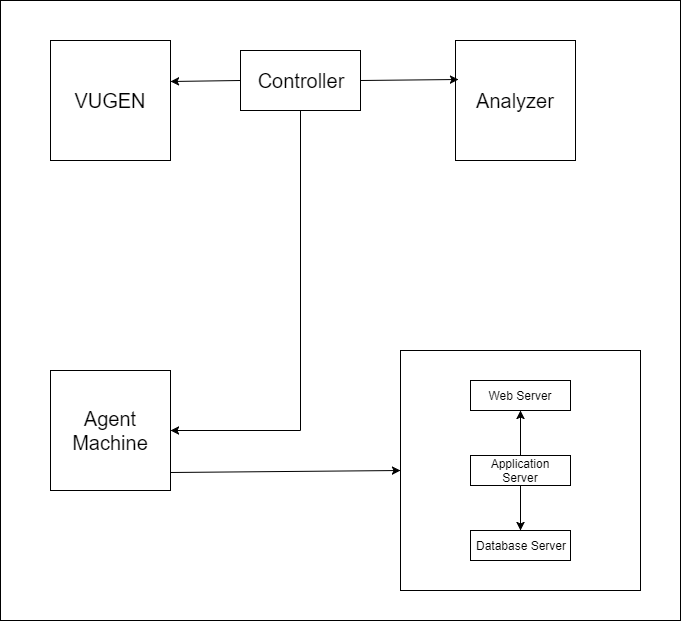
\includegraphics[width=120mm]{Loadrunner_architecture.png}
  \caption{Loadrunner Architecture \label{overflow}}
\end{figure}
\begin{itemize}
  \item \textbf{VUGEN} VUGen or Virtual User Generator is an IDE (Integrated Development Environment) or a rich coding editor. VUGen is used to replicate System Under Load (SUL) behaviour. VUGen provides a "recording" feature which records communication to and from client and Server in form of a coded script - also called VUser script.
  \paragraph{}
  \item \textbf{Controller} Once a VUser script is finalized, Controller is the main component which controls the Load simulation by managing, for example:
    \begin{itemize}
      \item How many VUsers to simulate against each business process or VUser Group
      \item Behaviour of VUsers (ramp up, ramp down, simultaneous or concurrent nature etc.)
      \item Nature of Load scenario e.g. Real Life or Goal Oriented or verifying SLA
      \item Which injectors to use, how many VUsers against each injector
      \item Collate results periodically
      \item IP Spoofing
      \item Error reporting
      \item Transaction reporting etc. 
    \end{itemize}
    \paragraph{}
  \item \textbf{Agents Machine/Load Generators/Injectors} LoadRunner Controller is responsible to simulate thousands of VUsers - these VUsers consume hardware resources for example processor and memory - hence putting a limit on the machine which is simulating them. Besides, Controller simulates these VUsers from the same machine (where Controller resides) and hence the results may not be precise. To address this concern, all VUsers are spread across various machines, called Load Generators or Load Injectors.
  \paragraph{}
  As a general practice, Controller resides on a different machine and load is simulated from other machines. Depending upon the protocol of VUser scripts and machine specifications, a number of Load Injectors may be required for full simulation. For example, VUsers for an HTTP script will require 2-4MB per VUser for simulation, hence 4 machines with 4 GB RAM each will be required to simulate a load of 10,000 VUsers.
  \paragraph{}
  \item \textbf{Analyzer} Once Load scenarios have been executed, the role of "Analysis" component comes in. During the execution, Controller creates a dump of results in raw form and contains information like, which version of LoadRunner created this results dump and what were configurations. All the errors and exceptions are logged in a Microsoft access database, named, output.mdb. The "Analysis" component reads this database file to perform various types of analysis and generates graphs.
  These graphs show various trends to understand the reasoning behind errors and failure under load; thus help figuring whether optimization is required in SUL, Server (e.g. JBoss, Oracle) or infrastructure.
\end{itemize}
\subsection{JMeter}
\end{document}
